\documentclass[12pt,letterpaper]{article}
\usepackage{graphicx,textcomp}
\usepackage{natbib}
\usepackage{setspace}
\usepackage{fullpage}
\usepackage{color}
\usepackage[reqno]{amsmath}
\usepackage{amsthm}
\usepackage{fancyvrb}
\usepackage{amssymb,enumerate}
\usepackage[all]{xy}
\usepackage{endnotes}
\usepackage{lscape}
\newtheorem{com}{Comment}
\usepackage{float}
\usepackage{hyperref}
\newtheorem{lem} {Lemma}
\newtheorem{prop}{Proposition}
\newtheorem{thm}{Theorem}
\newtheorem{defn}{Definition}
\newtheorem{cor}{Corollary}
\newtheorem{obs}{Observation}
\usepackage[compact]{titlesec}
\usepackage{dcolumn}
\usepackage{tikz}
\usetikzlibrary{arrows}
\usepackage{multirow}
\usepackage{xcolor}
\newcolumntype{.}{D{.}{.}{-1}}
\newcolumntype{d}[1]{D{.}{.}{#1}}
\definecolor{light-gray}{gray}{0.65}
\usepackage{url}
\usepackage{listings}
\usepackage{color}

\definecolor{codegreen}{rgb}{0,0.6,0}
\definecolor{codegray}{rgb}{0.5,0.5,0.5}
\definecolor{codepurple}{rgb}{0.58,0,0.82}
\definecolor{backcolour}{rgb}{0.95,0.95,0.92}

\lstdefinestyle{mystyle}{
	backgroundcolor=\color{backcolour},   
	commentstyle=\color{codegreen},
	keywordstyle=\color{magenta},
	numberstyle=\tiny\color{codegray},
	stringstyle=\color{codepurple},
	basicstyle=\footnotesize,
	breakatwhitespace=false,         
	breaklines=true,                 
	captionpos=b,                    
	keepspaces=true,                 
	numbers=left,                    
	numbersep=5pt,                  
	showspaces=false,                
	showstringspaces=false,
	showtabs=false,                  
	tabsize=2
}
\lstset{style=mystyle}
\newcommand{\Sref}[1]{Section~\ref{#1}}
\newtheorem{hyp}{Hypothesis}

\title{Problem Set 2}
\author{Applied Stats / Quant Methods 1}
\date{Lucas de Melo Prado / Due: October 16, 2022}

\begin{document}
	
	\maketitle
	
\section*{Instructions}
	
	\begin{itemize}
	
		\item Please show your work! You may lose points by simply writing in the answer. If the problem requires you to execute commands in \texttt{R}, please include the code you used to get your answers. Please also include the \texttt{.R} file that contains your code. If you are not sure if work needs to be shown for a particular problem, please ask.
	
		\item Your homework should be submitted electronically on GitHub.
	
		\item This problem set is due before 23:59 on Sunday October 16, 2022. No late assignments will be accepted.
	
		\item Total available points for this homework is 80.
	
	\end{itemize}
	
	\vspace{.5cm}

\section*{Question 1 (40 points): Political Science}
	
	\vspace{.25cm}
		
	The following table was created using the data from a study run in a major Latin American city.\footnote{Fried, Lagunes, and Venkataramani (2010). ``Corruption and Inequality at the Crossroad: A Multimethod Study of Bribery and Discrimination in Latin America. \textit{Latin American Research Review}. 45 (1): 76-97.} As part of the experimental treatment in the study, one employee of the research team was chosen to make illegal left turns across traffic to draw the attention of the police officers on shift. Two employee drivers were upper class, two were lower class drivers, and the identity of the driver was randomly assigned per encounter. The researchers were interested in whether officers were more or less likely to solicit a bribe from drivers depending on their class (officers use phrases like, ``We can solve this the easy way'' to draw a bribe). The table below shows the resulting data.

	\newpage

	\begin{table}[h!]
		\centering
		\begin{tabular}{l | c c c }
			& Not Stopped & Bribe requested & Stopped/given warning \\
			\\[-1.8ex] 
			\hline \\[-1.8ex]
			Upper class & 14 & 6 & 7 \\
			Lower class & 7 & 7 & 1 \\
			\hline
		\end{tabular}
	\end{table}

	\begin{enumerate}
	
		\item [(a)]
		Calculate the $\chi^2$ test statistic by hand/manually (even better if you can do "by hand" in \texttt{R}).\\
		
		To calculate $\chi^2$ in \texttt{R}, we first import the data and create a contingency table:
		
				\lstinputlisting[language=R, firstline=12, lastline=19]{PS02_answersLucasDeMeloPrado.R}
		
		Then, we follow the steps to perform the test.\\
		
		\textbf{1. Assumption.} Data collection was randomized and most frequencies ($>75\%$) are $\ge 5$\\
		
		\textbf{2. Hypotheses.} For the \textit{null hypothesis}, we consider that variables are statistically independent: $$H_0: f_0 = f_e \text{ or } H_0: f_0 - f_e=0.$$
		
		The \textit{alternative hypothesis} is that variables are statistically dependent: $$H_a: f_0 \neq f_e.$$
		
		\textbf{3. Chi-squared test statistic.} To perform the chi-squared test, we first need to find the expected frequencies ($f_e$) for each cell were the null hypothesis true:
			
			$$f_e = \frac{\text{(row total)} \cdot \text{(column total)}}{\text{overall sample size}}.$$
			
			\lstinputlisting[language=R, firstline=21, lastline=27]{PS02_answersLucasDeMeloPrado.R}
		
		We can summarize the values of observed frequencies ($f_0$) and expected frequencies ($f_e$) in the following table:
		
		\begin{table}[H]
			\centering
			\begin{tabular}{l | c c c }
				& Not Stopped & Bribe requested & Stopped/given warning \\
				\\ [-1.8ex] 
				\hline \\[-1.8ex]
 				Upper class	& $f_0=14$ & $f_0=6$ & $f_0=7$ \\
 							& $f_e=13.5$ & $f_e=8.36$ & $f_e=5.14$ \\
 				\\ [-1.8ex]
				Lower class	& $f_0=7$ & $f_0=7$ & $f_0=1$ \\
							& $f_e=7.5$ & $f_e=4.64$ & $f_e=2.86$ \\
				\\[-1.8ex]
				\hline
			\end{tabular}
		\end{table}

		Finally, we calculate $\chi^2$:
		
			$$\chi^2 = \sum{\frac{(f_o-f_e)^2}{f_e}}$$
		
			$$\chi^2 = \frac{(14-13.5)^2}{13.5} + \frac{(6-8.36)^2}{8.36} + \frac{(7-5.14)^2}{5.14} + \frac{(7-7.5)^2}{7.5} + \frac{(7-4.64)^2}{4.64} + \frac{(1-2.86)^2}{2.86}$$
		
			$$\chi^2 = 3.79$$
		
			\lstinputlisting[language=R, firstline=29, lastline=30]{PS02_answersLucasDeMeloPrado.R}
		
		\vspace{.5cm}
	
		\item [(b)]
		Now calculate the p-value from the test statistic you just created (in \texttt{R}).\footnote{Remember frequency should be $>5$ for all cells, but let's calculate the p-value here anyway.}  What do you conclude if $\alpha = 0.1$?\\
		
		\textbf{4. P-value.}
		
			\lstinputlisting[language=R, firstline=32, lastline=34]{PS02_answersLucasDeMeloPrado.R}
		
		$$df = \text{(number of rows - 1)} \cdot \text{(number of columns - 1)} = (2-1) \cdot (3-1) = 2$$
		$$p = 0.15$$
		
		\textbf{5. Conclusion.} For $\alpha = 0.1$, \textit{we do not have enough evidence to reject the null hypothesis}, according to which variables are statistically independent.
		
		\newpage
	
		\item [(c)] Calculate the standardized residuals for each cell and put them in the table below.\\
		
		To calculate the standardized residuals (z) for each cell, we use this formula:
		
		$$z = \frac{f_0 - f_e}{se} = \frac{f_0 - f_e}{\sqrt{f_e \cdot (1-\text{row proportion}) \cdot (1-\text{column proportion})}}$$\\
		
			\lstinputlisting[language=R, firstline=39, lastline=57]{PS02_answersLucasDeMeloPrado.R}
		
		These are the results we obtained:
		
		\begin{table}[h]
		\centering
			\begin{tabular}{l | c c c }
				& Not Stopped & Bribe requested & Stopped/given warning \\
				\\[-1.8ex] 
				\hline \\[-1.8ex]
				Upper class  & 0.32 & -1.64 & 1.52 \\
				\\[-1.8ex]
				Lower class & -0.32 & 1.64 & -1.52 \\
			\end{tabular}
		\end{table}
		
		\vspace{.5cm}
	
		\item [(d)] How might the standardized residuals help you interpret the results?\\
		
		Standardized residuals represent the number of standard errors the residuals $(f_0 - f_e)$ fall from the expected value if the null hypothesis is true, i.e., $f_0-f_e=0$. As standard residuals behave like a normal distribution, large standard residuals (below $-3$ or above $3$) would be strong evidence against $H_0$.
		
		However, in the present case, all standard residuals are between -2 and 2. This reinforces the high p-value we have already found. Therefore, standard residuals do not allow us to reject the null hypothesis either.
	
	
	\end{enumerate}

\newpage

\section*{Question 2 (40 points): Economics}

	Chattopadhyay and Duflo were interested in whether women promote different policies than men.\footnote{Chattopadhyay and Duflo. (2004). ``Women as Policy Makers: Evidence from a Randomized Policy Experiment in India. \textit{Econometrica}. 72 (5), 1409-1443.} Answering this question with observational data is pretty difficult due to potential confounding problems (e.g. the districts that choose female politicians are likely to systematically differ in other aspects too). Hence, they exploit a randomized policy experiment in India, where since the mid-1990s, $\frac{1}{3}$ of village council heads have been randomly reserved for women. A subset of the data from West Bengal can be found at the following link: \url{https://raw.githubusercontent.com/kosukeimai/qss/master/PREDICTION/women.csv}\\

	\noindent Each observation in the data set represents a village and there are two villages associated with one GP (i.e. a level of government is called "GP"). Figure~\ref{fig:women_desc} below shows the names and descriptions of the variables in the dataset. The authors hypothesize that female politicians are more likely to support policies female voters want. Researchers found that more women complain about the quality of drinking water than men. You need to estimate the effect of the reservation policy on the number of new or repaired drinking water facilities in the villages.
	
	\begin{figure}[h!]
		\caption{\footnotesize{Names and description of variables from Chattopadhyay and Duflo (2004).}}
		\vspace{.5cm}
		\centering
		\label{fig:women_desc}
		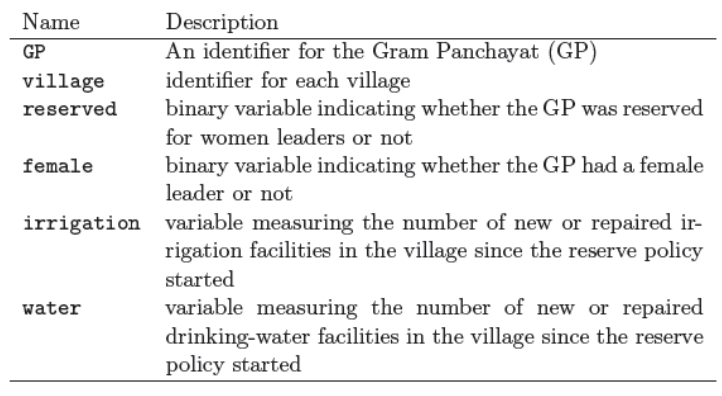
\includegraphics[width=0.8\textwidth]{women_desc.png}
	\end{figure}
	
	\vspace{.5cm}

	\newpage
	
	\begin{enumerate}
	\item [(a)] State a null and alternative (two-tailed) hypothesis. 
	
	For the \textit{null hypothesis}, we assume that there is no association between the two variables, \textit{i.e.}, between the reservation policy and the number of new or repaired drinking water facilities in the village:
	$$H_0: \beta = 0$$
	
	For the \textit{alternative hypothesis}, we assume that there is some association between these two variables:
	$$H_a: \beta \neq 0$$
	
	\vspace{0.5cm}
	
	\item [(b)] Run a bivariate regression to test this hypothesis in \texttt{R} (include your code!).
	
	\textbf{1. Assumptions.} We work with \textit{four} assumptions: 1) data were randomly collected; 2) the association between variables is linear; 3) the values of the response variable for each value of the explanatory variable follow a normal distribution; and 4) all distributions of the response variable have the same standard deviation.
	
	\textbf{2. Hypothesis.} $H_0: \beta = 0$; $H_a: \beta \neq 0$.
	
	\textbf{3. Test statistic.} For the test statistic of $\beta$, we perform a t-test. This test depends on the prediction equation for the linear function $(\hat{y}=a+bx)$, as well as on the standard error of $\beta$ ($se_\beta$), which, in turn, depends on the standard deviation of $\beta$ ($s_\beta$).
	
	First, we establish the \textit{prediction equation} ($\hat{y}=a+bx$):
	
	$$b = \frac{\sum (x-\bar{x})(y-\bar{y})}{\sum (x-\bar{x})^2} = \frac{664.10}{71.78} = 9.25$$
	
	$$a = \bar{y} - b\bar{x} = 17.84 - 9.25 \cdot 0.33 = 14.74$$
	
	$$\hat{y} = 14.74 + 9.25x$$
	
		\lstinputlisting[language=R, firstline=66, lastline=74]{PS02_answersLucasDeMeloPrado.R}
	
	Then, we calculate the \textit{standard deviation} ($s_\beta$) and the \textit{standard error} ($se_\beta$) of $\beta$:
	
	$$s_\beta = \sqrt{\frac{SSE}{n-2}} = \sqrt{\frac{\sum(y-\hat{y})^2}{n-2}} = \sqrt{\frac{357,956.3}{320}} = \sqrt{1,118.61} = 33.44$$
	
	$$se_\beta = \frac{s_\beta}{\sqrt{\sum (x-\bar{x})^2}} = \frac{33.44}{8.47} = 3.95$$
	
		\lstinputlisting[language=R, firstline=76, lastline=78]{PS02_answersLucasDeMeloPrado.R}
	
	Finally, we perform the \textit{t-test} ($t$):
	
	$$t = \frac{b-\beta_0}{se} = \frac{9.25}{3.95} = 2.34$$

		\lstinputlisting[language=R, firstline=80, lastline=81]{PS02_answersLucasDeMeloPrado.R}
		
	\textbf{4. P-value.} For a two-tailed test, $p=0.019$.

		\lstinputlisting[language=R, firstline=83, lastline=84]{PS02_answersLucasDeMeloPrado.R}
	
	Finally, we check our results:

		\lstinputlisting[language=R, firstline=86, lastline=87]{PS02_answersLucasDeMeloPrado.R}

	\item [(c)] Interpret the coefficient estimate for reservation policy.
	
	Depending on the established significance level ($\alpha$), we can draw different conclusions from the test. For a more demanding $\alpha=0.01$, $p=0.019$ does not provide enough evidence to reject the null hypothesis. However, for $\alpha=0.05$, the test allows the rejection of the null hypothesis.
	
	If we assume $\alpha=0.05$ and, therefore, reject $H_0$, then the association between the reservation policy ($x$) and the number of new or repaired drinking water facilities ($y$) is positive ($b>0$). The regression line intercepts the y-axis at $a=14.74$, and $y$ increases $b=9.25$ for each one-unit increase in $x$.

	\end{enumerate}

\end{document}
